
%% bare_conf.tex
%% V1.3
%% 2007/01/11
%% by Michael Shell
%% See:
%% http://www.michaelshell.org/
%% for current contact information.
%%
%% This is a skeleton file demonstrating the use of IEEEtran.cls
%% (requires IEEEtran.cls version 1.7 or later) with an IEEE conference paper.
%%
%% Support sites:
%% http://www.michaelshell.org/tex/ieeetran/
%% http://www.ctan.org/tex-archive/macros/latex/contrib/IEEEtran/
%% and
%% http://www.ieee.org/

\documentclass[10pt, conference]{IEEEtran}

\usepackage{booktabs}
\usepackage{cite}
\usepackage{color}
\usepackage{enumerate}
\usepackage[utf8]{inputenc}
\usepackage{tikz}
\usepackage{multicol}
\usepackage{multirow}
\usepackage{subcaption}
\usepackage[skip=0pt]{caption}


%\usepackage[brazil]{babel}
%\usepackage[cmex10]{amsmath}
%\usepackage{algorithmic}
%\usepackage{array}
%\usepackage{mdwmath}
%\usepackage{mdwtab}
%\usepackage{eqparbox}
%\usepackage[tight,footnotesize]{subfigure}
%\usepackage[caption=false]{caption}
%\usepackage[font=footnotesize]{subfig}
%\usepackage[caption=false,font=footnotesize]{subfig}
%\usepackage{fixltx2e}
%\usepackage{stfloats}
\usepackage{url}

\makeatletter
\setlength{\@fptop}{0pt}
\makeatother

\newif\ifComments

% To turn comments OFF simply comment out the \Commentstrue line
\Commentstrue

\ifComments
\newcommand{\luiz}[1]{\noindent\textcolor{orange}{LUIZ: {#1}}}
\newcommand{\mario}[1]{\noindent\textcolor{cyan}{MARIO: {#1}}}
\newcommand{\rem}[1]{\noindent\textcolor{magenta}{REMOVED: {#1}}}
\newcommand{\new}[1]{\noindent\textcolor{blue}{NEW: {#1}}}
\newcommand{\rev}[1]{\noindent\textcolor{red}{REVISE: {#1}}}
\else
\newcommand{\luiz}[1]{}
\newcommand{\mario}[1]{}
\newcommand{\rem}[1]{}
\newcommand{\new}[1]{#1}
\newcommand{\rev}[1]{#1}
\fi

% correct bad hyphenation here
\hyphenation{}
\usetikzlibrary{shapes.geometric, arrows}

\tikzstyle{activity} = [rectangle, rounded corners, minimum width=5cm, minimum 
height=1cm,text centered, draw=black, fill=white]
\tikzstyle{io} = [trapezium, trapezium left angle=70, trapezium right angle=110, minimum width=3cm, minimum height=1cm, text centered, draw=black, fill=blue!30]
\tikzstyle{process} = [rectangle, minimum width=3cm, minimum height=1cm, text centered, text width=3cm, draw=black, fill=orange!30]
\tikzstyle{decision} = [diamond, minimum width=3cm, minimum height=1cm, text centered, draw=black, fill=green!30]
\tikzstyle{arrow} = [thick,->,>=stealth]
\tikzstyle{line} = [draw, -latex']


\begin{document}

\title{Machine Learning Based Prediction of Change Request Severity Level: Experimental Results}

\author{\IEEEauthorblockN{Author1}
\IEEEauthorblockA{Affiliation1}
\and
\IEEEauthorblockN{Author2}
\IEEEauthorblockA{Affiliation2}
}

\maketitle

\begin{abstract}
In the context of Change Request (CR) systems, the severity level of a change request is considered a critical variable when planning software maintenance activities, indicating how soon a CR needs to be addressed. However, the severity level assignment remains primarily a manual process, mostly depending on the experience and expertise of the person who has reported the CR. In this paper, we present preliminary findings of ongoing research aimed to predict the severity level of a CR by analyzing its long description, using text mining techniques and Machine Learning (ML) algorithms. Best results were obtained with a classifier based on the Random Forest ML algorithm. This classifier can predict whether the severity level will change (accuracy of 93.7\%) and if it will increase or decrease (accuracy of 93.4\%). Preliminary results have shown that its accuracy was 68.1\% when predicting the final severity level in an imbalanced data scenario, which is a value similar to the literature. We have also shown that the classical measurements do not help deciding if the ML approach will bring any benefit to the user, and have proposed an alternative measuring approach to address this issue.

\end{abstract}

\begin{IEEEkeywords}
software maintenance; change request systems; machine learning; random forest.
\end{IEEEkeywords}


% For peer review papers, you can put extra information on the cover
% page as needed:
% \ifCLASSOPTIONpeerreview
% \begin{center} \bfseries EDICS Category: 3-BBND \end{center}
% \fi
%
% For peerreview papers, this IEEEtran command inserts a page break and
% creates the second title. It will be ignored for other modes.
\IEEEpeerreviewmaketitle




\section{Introduction}
Change Request (CR) systems have played a major role in maintenance process in many software development settings, both in Close Source Software (CSS) and in Open Source Software (OSS) scenarios. This is specially true in OSS, which is characterized by the existence of many of users and developers with different levels of expertise spread out around the world, who might create or be responsible for dealing with several CRs\cite{Cavalcanti2014}. 

A user interacts with a CR system often through a simple mechanism called CR form. This form enables him to request changes, to report bugs or to ask for support in a software product\cite{Sommerville2010}. Initially, he or she should inform a short description, a long description, a type (e.g. bug, new feature, improvement, and task) and an associated severity level (e.g. blocker, critical, major, minor and trivial). Subsequently, a development team member will review this request and, case it is not refused for some reason (e.g. request duplication), he or she will complete the information in CR form, indicating, for example, its priority and assigning the person responsible for the CR. 

The severity level information is recognized as a critical variable in the equation to estimate a prioritization of CRs \cite{Tian2012}. It defines how soon the CR needs to be addressed\cite{Lamkanfi2010}. However, the severity level assignment remains mostly a manual process which relies only on the experience and expertise of the person who has opened the CR \cite{Cavalcanti2014, Tian2012, Lamkanfi2010}. As a consequence, it is a process with high degree of subjectivity, and it may be quite error-prone. 

The number of CRs in large and medium software OSS projects \cite{Lamkanfi2011} is frequently very large. Severity level shifts throughout CR lifecycle may have an adverse effect on the planning of maintenance activities. For example, the maintenance team could be assigned to address less significant CRs before  most important ones. There has been reports of efforts to implement intelligent software assistants to help developers and maintenance personnel in defining more accurately the field values in a CR form. Currently, Machine Learning techniques have become a popular method to address this issue and there is quite a few publications in this area in the literature \cite{Cavalcanti2014}. 

Machine Learning (ML) techniques have been successfully applied in solving real problems in many areas of knowledge, including those related to CR systems, such as duplication and assignment of CR\cite{Cavalcanti2014}. However, the accuracy of ML algorithms may be affected by imbalanced datasets \cite{Chawla2009} \textemdash  a recurring critical problem in CR repositories\cite{Tian2015}. For example, more than 60\% of CRs may have a ``major'' severity level. In addition to this problem, most publications are still focused in predicting the severity level of CRs and none of them have been implemented into popular tools like as Bugzilla, Jira and Redmine.\cite{Cavalcanti2014}. Furthermore, many have used proprietary and/or not public ML algorithms. Therefore, there is still a clear need of advances in this knowledge area, specially broadening the reach of research questions and including more popular and open OSS and ML algorithms.


In this context, the general purpose of our research is to develop an intelligent ML based assistant to help developers and maintenance personnel in the OSS maintenance activies. In this current article, our specific goals are:

\begin{enumerate}[$G_1:$]
\item Evaluate the performance of traditional ML algorithms in the prediction of CR severity level; 
\item Identify a suitable algorithm to perform such prediction in a scenario where imbalanced data is natural;
\item Propose a new metric to compare the performance of the software ML system and the user, in predicting or assigning the final CR Level.
\end{enumerate}

In order to meet these goals, this research works with the following research questions, regarding CR severity level during its lifecycle:

\begin{enumerate}[$RQ_1:$]
  \item \textit{Will the CR severity level change?}
  \item \textit{Will the CR severity level increase, decrease or remain the same}? 
  \item \textit{What is the prediction for the final CR severity level?}
  \item \textit{How ML predictions compare to user prediction?} 
\end{enumerate}


The contributions of our reasearch are:


\begin{itemize}
  \item Indicate the performance of three ML algorithms in multi category classifiers on imbalanced scenario. 
  \item Propose a new way to measure the performance of ML algorithms taking into account the user prediction.
  \item Extend published results to include new FLOSS, new open ML algorithms, and new CR Repositories.
\end{itemize}


The article is organized as follows. Section \ref{sec:relatedwork} presents related work that are relevant to our research. Section \ref{sec:background} provides the information background about CR systems, text mining and machine learning techniques necessary to understand our approach. Section \ref{sec:experiment} describes our work. Section \ref{sec:discussion} presents final findings and discussion. Finally, Section \ref{sec:conclusion} present  conclusions and  future work.


\section{Related Work}\label{sec:relatedwork} 

This section presents relevant articles in the area of mining open system repositories, aiming at extracting data and using ML techniques to predict several maintenance properties. 

Menzies\cite{Menzies2008} have developed a method, named SEVERIS (SEVERity ISsue assessment), for evaluating the severity of CRs. SEVERIS is based on stablished data and text mining techniques. The method was applied to predict CR severity level in five projects managed by the Project and Issue Tracking System (PITS), an issue tracker system used by NASA (Stratified F-measures by severity level in the range: (2) 78\%-86\%; (3) 68\%-98\%; (4) 86\%-92\%).


Lamkanfi et al.\cite{Lamkanfi2010} have developed an approach to predict if severity of bug report is non-severe (severity levels: 1 or 2) or severe (severity levels: 4 or 5) based on text mining algorithms (tokenization, stop word removal, stemming) and on the Naïve Bayes machine learning algorithm. They have validated their approach with data from three open source project (Mozilla, Eclipse, and GNOME). The article reports that a training set with approximately 500 CRs per severity level is sufficient to make predictions with reasonable accuracy (precision and recall in the range 0.65-0.75 with Mozilla and Eclipse; 0.70-0.85 with GNOME).

Valdivia et al.\cite{ValdiviaGarcia2014} have characterized blocking bugs in six open source projects and proposed a model to predict them. Their model was composed of 14 distinct factors or features (e.g. the textual description, location the bug is found in and the people involved with the bug). Based on these factors they have build decision trees for each project to predict whether a bug will be a blocking bug or not (F-measures in the range 15-42\%).

Tian et al.\cite{Tian2012} have develop a method to predict the severity level of new CRs based on similar CRs reported in the past. The comparison between old and new CRs was implemented by the BM25 similarity function. This method was applied to Mozilla, Eclipse and OpenOffice projects over more than 250,000 CR extracted from Bugzilla (F-measure in the range 13.9-65.3\% for Mozilla; 8.6-58\% for Eclipse; and 12.3-74\% for OpenOffice). 


\section{BACKGROUND} \label{sec:background} 
 

This section briefly comments of basic concepts necessary to comprehend this research area, namely CR Systems, Text Mining, Machine Learning, and ML evaluation metrics.

Data used in this research area are usually extracted from the so called CR Systems, or Gug Tracking Systems. Popular CR Systems are Bugzilla, Jira, and Redmine \cite{Tian2012}. Additional information can be found in \cite{Pressman2009}.

Two techniques are frequently used in this research area: Text Mining  \cite{Feldman2007} \cite{Williams2011} and Machine Learning (ML) \cite{Williams2011} \cite{Surya2016} \cite{Russell2010} \cite{Breiman2001}. Detailing of these techniques are outside the scope of this paper.

Finally, it is worth mentioning the specific metrics used in this research are for assessing prediction performance. The three most common performance measures for evaluating the accuracy of classification algorithms are precision, recall, and F-measure, described as follows \cite{Facelli2015} \cite{Zhao2013}:

\textbf{Recall}. Recall is the number of True Positives (TP) divided by the number of True Positives (TP) and of False Negatives (FN), where the TP and FN values are derived from the confusion matrix. A low recall indicates many false negatives.

\textbf{Precision}. Precision is the number of True Positives (TP) divided by the number of True Positives and False Positives (FP). A low precision can also indicate a large number of false positives.

\textbf{F-measure}. F-measure conveys the balance between precision and recall, and can be calculated as their harmonic mean. 



\section{Experiment} \label{sec:experiment}
This section describes the experiment conducted to address the Research Questions. As in typical methodologies used in ML studies, it comprises the followint steps: Data Collection (\ref{subsec:collection}), Data Preprocessing (Section \ref{subsec:preprocessing}), and Training and Testing (Section \ref{subsec:training}).

\subsection{Data Collection} 	\label{subsec:collection}
This step in the experimental research encompasses sellecting a FLOSS to serve as the data source, studying and interpreting its data structure, and finally extracting relevant data from its repository (feature extraction). In this research, Hadoop, Linux, and Mozilla Open Systems were considered as potential Open Source Systems to study. In a first approximation, Hadoop was sellected as a data source of CR records, due to the fact it is open, well stablished, has a considerable number of CRs already registered, uses standard repositories, and was under study by other researchers in our research group. According to [hadoop.apache.org], HADOOP is a ``framework that allows for the distributed processing of large data sets across clusters of computers using simple programming models''. It is considered a specialized and complex OSS project with many users with different levels of expertise. Its CR repository allows for access to all CR contents in XML format. Everything is available (except change history), from CR long description field (with lines with few characters to ones with many lines), including code snippets and exception stack trace.

CRs in HADOOP are stored in a Jira based repository [\url{https://www.atlassian.com/software/jira}]. Two steps are used to perform data extraction from HADOOP web site[\url{http://issues.apache.org}]: (i) copying CR basic data (e.g. status and resolution) from XML contents; and (ii) copying CR changes history from external HTML pages (this may be important for learning). About 10\% of the CRs collected in this process changed their level of severity at least once.


CR record data from February 01, 2006 to January 18, 2017 was collected.  Only requests from the common module (identifier = HADOOP-*)were considered for retrieval. The total number of CR records retrieved after preprocessing was 7129. 

\begin{figure*}[!t]
  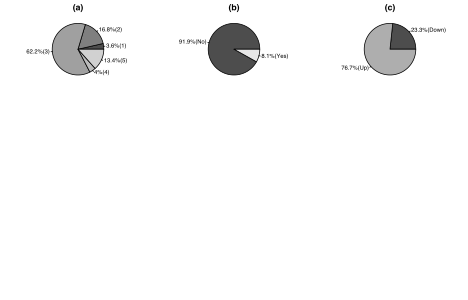
\includegraphics[scale=0.9]{figures/ds_distribution.pdf}    % ordem SEMPRE: include, caption, label
  \caption{Dataset distribution.}
  \label{fig:ds_distribution}
\end{figure*}



Figure \ref{fig:ds_distribution} shows how the 7129 retrieved CR records were distributed in terms of severity level and severity level change. Figure \ref{fig:ds_distribution}(a) shows the severity level distribution: 3.6\% have severity 1 (trivial); 16.8\% have severity 2 (minor); 62.2\% have severity 3 (major), 4.0\% have severity 4 (critical), and 13.4\% have severity 5 (blocker). Figure \ref{fig:ds_distribution}(b) shows that only 8.1\% have changed their severities levels during the CR lifecycle. Finally, Figure \ref{fig:ds_distribution}(c) reveals that of these 8.1\% CRs which changed their severity, 23.3\% decreased it, and 76.7\% increased it. One can see that this dataset is clearly imbalanced, posing addicional difficulty to the application of the ML methodology. 

\subsection{Preprocessing} 	\label{subsec:preprocessing}

The raw data previously collected from the HADOOP CR repository was not properly structured to serve as input to ML algorithms, it was in tidy data format \cite{DeJonge2013}. The classical way to address this problem is to run preprocessing procedures to extract, organize and structure relevant information out of the raw data. Specific scripts were written in R language to acomplish this. Preprocessing tasks were executed as follows:  

\begin{itemize}
 \item Extraction of relevant features: key, type, status, resolution status, and long description of CRs; 
 \item Filtering CRs with status equals to Closed and resolution equals to Fixed and Implemented. 
 \item Merging CR features with their change history data. This additional information allows for the identification of CRs that have changed severity level during the CR lifecycle, and furthermore, if they have changed for better (decrease) or worse (increase).
 \item Performing text mining in the long description field to identify the 100 most frequent words. This information is then converted into features for each CR.
 \item Sorting the CRs in ascending chronological date. 
\end{itemize}


\subsection{Training and testing}  	\label{subsec:training}

Training and testing steps start with partitioning the already preprocessed dataset in two disjoint subsets: a subset for training, with 60\% of the CRs, and a subset for testing, with the remaining 40\% of the CRs. Three classical sampling approaches, random, proportional, and uniform, were analyzed to select the training set. Best results were obtained with the random sampling technique. In the training phase, we have used the 3-fold cross-validation technique \cite{Zhao2013} to choose the best values for hyperparameters for each classifier algorithm to use them in the test phase. 


\section{Findings and Discussions}  \label{sec:discussion}

\subsection{RQ1: Will the CR severity level change?}

The RQ1 is a simple binary problem, i.e., a question whose answer is true or false. Table \ref{tab:metrics_for_rq1} shows the performance (in percentage) of the classifiers to predict the response to this issue.


\begin{table}[!ht]
	\renewcommand{\arraystretch}{1.5}
	\caption{Classifiers Performances on RQ1.}
	\label{tab:metrics_for_rq1}
	\centering
	\begin{tabular}{|l|c|c|c|}
		\hline
		Classifier & Precision & Recall & F-measure\\
		\hline 
		Neural Net. & 93.381 & 98.015 & 95.642\\
		\hline
		Random Forest & 93.801 & 99.923 & 96.765\\
        \hline
		SVM & 93.727 & 99.809 & 96.627 \\
		\hline
		
	\end{tabular}
\end{table}

We tested the classifiers with 2851 (40\% of 7129) CR: 2620 have changed their severity level, and 231 haven't changed their severity level. We can observe that the three classifiers performed very closely. However, the Random Forest classifier have achieved a F1-Measure somewhat better than the two others. 

Regarding the Random Forest classifier we have done one step further, we have investigated its performance relating to the number of hits and errors made in answer to RQ1. Figure \ref{fig:rf_performance_for_q1q2} indicates that its accuracy was 93.681\% ($2676 / 2851$). This performance is better than others \cite{Lamkanfi2010, ValdiviaGarcia2014} reported in the literature (see Table \ref{tab:metrics_for_rq}).

\begin{figure}[!hbt]
  \includegraphics[scale=1.0]{figures/rf_performance_for_q1q2.pdf}
  \caption{Performance of Random Forest for RQ1 and RQ2.}
  \label{fig:rf_performance_for_q1q2}
\end{figure}

\subsection{RQ2: Will the CR severity level increase, decrease or remain the same?}

The RQ2 poses a problem more difficult than a previous question. It is a question with three possible responses related to severity level: (-1) it has decreased; (0)  it has remained; and (1) it has increased. Table \ref{tab:metrics_for_rq2} shows the performance (in percentage) of the classifiers to predict the response to this issue.


\begin{table}[!ht]
	% increase table row spacing, adjust to taste
	\renewcommand{\arraystretch}{1.5}
	\caption{Classifiers Performance on RQ2.}
	\label{tab:metrics_for_rq2}
	\centering
	\begin{tabular}{l|c|c|c|c|}
		\cline{2-5}
		& Class & Precision & Recall & F-measure\\
		\hline\cline{2-5}
        \multicolumn{1}{ |c| }{\multirow{4}{*}{\rotatebox[origin=c]{90}{\scriptsize{Neural Net.}}}} & -1 & 3.703 & 28.571 & 6.557\\
		\cline{2-5}
		\multicolumn{1}{ |c| }{} & 0 & 97.663 & 93.357 & 95.447\\
		\cline{2-5}
		\multicolumn{1}{ |c| }{} & 1 & 22.598 & 38.461 & 28.469\\
		\cline{2-5} 
		\multicolumn{1}{ |c| }{} & Average & 41.311 & 53.463 & 43.491 \\
		\hline\hline 
		\multicolumn{1}{ |c| }{\multirow{4}{*}{\rotatebox[origin=c]{90}{\scriptsize{Random Forest}}}} & -1 & 13.111 & 85.714 & 19.672\\
		\cline{2-5}
		\multicolumn{1}{ |c| }{} & 0 & 99.923 & 93.500 & 96.605\\
		\cline{2-5}
		\multicolumn{1}{ |c| }{} & 1 & 28.598 & 90.652 & 46.199\\
		\cline{2-5} 
		\multicolumn{1}{ |c| }{} & Average & 47.210 & 89.955 & 54.158 \\

		\hline\hline 
		\multicolumn{1}{ |c| }{\multirow{4}{*}{\rotatebox[origin=c]{90}{\scriptsize{SVM}}}} 		
		& -1 & 12.962 & 70.000 & 21.875\\
		\cline{2-5}
		\multicolumn{1}{ |c| }{} & 0 & 99.923 & 93.902 & 96.819\\
		\cline{2-5}
		\multicolumn{1}{ |c| }{} & 1 & 27.118 & 90.566 & 41.739\\
		\cline{2-5} 
		\multicolumn{1}{ |c| }{} & Average & 46.667 & 84.822 & 53.477 \\
		
		
		\hline
		 
	\end{tabular}
\end{table}


We have tested the classifiers with 2851 (40\% of 7129) CRs. Only now, we have three predicting situations: 2620 haven't changed their severity level, 177 have increased their severity level, and 54 have decreased their severity level. We can observe in the Table \ref{tab:metrics_for_rq2} which the classifiers also performed very closely as question 1. However, the Random Forest classifier have achieved F-measure somewhat better than the two others.

As in RQ1, we have done a step further regarding the best classifier. We have investigated its performance, observing the number of correct and incorrect answers on the test dataset as a whole. Figure \ref{fig:rf_performance_for_q1q2} indicates that its accuracy was 93.440\% ($ 2664 / 2851$) in the RQ2 prediction. This performance is better than \cite{Tian2012} and worse than \cite{Menzies2008} (see Table \ref{tab:metrics_for_rq}).

%\begin{figure}[!hbt]
%   \label{fig:rf_performance_for_q2}
%  \includegraphics{figures/rf_performance_for_q2.pdf}
%  \caption{Performance of Random Forest for RQ2.}
%\end{figure}

\subsection{RQ3: What is the prediction for the final CR severity level?}

The RQ3 is a problem much harder than other two. It is a question with five responses related to severity level: (1) trivial; (2) minor; (3) major; (4) critical; and (5) blocker. Table \ref{tab:metrics_for_rq3} shows the performance (in percentage) of the classifiers to predict the response to this issue.


\begin{table}[!ht]
	% increase table row spacing, adjust to taste
	\renewcommand{\arraystretch}{1.5}
	\caption{Classifiers Performance on RQ3.}
	\label{tab:metrics_for_rq3}
	\centering
	\begin{tabular}{l|c|c|c|c|}
		\cline{2-5}
		& Class & Precision & Recall & F-measure\\
		\hline\cline{2-5}
        \multicolumn{1}{ |c| }{\multirow{6}{*}{\rotatebox[origin=c]{90}{\scriptsize{Neural Net.}}}} & 1 & 4.950 & 29.411 & 8.474\\
		\cline{2-5}
		\multicolumn{1}{ |c| }{} & 2 & 18.997 & 34.469 & 24.495\\
		\cline{2-5}
		\multicolumn{1}{ |c| }{} & 3 & 88.726 & 66.273 & 75.873\\
		\cline{2-5} 
		\multicolumn{1}{ |c| }{} & 4 & 16.964 & 37.254 & 23.312\\
		\cline{2-5} 
		\multicolumn{1}{ |c| }{} & 5 & 17.015 & 46.099 & 24.856\\
		\cline{2-5} 
		\multicolumn{1}{ |c| }{} & Average & 29.330 & 39.606 & 31.402 \\
		\hline\hline 
		\multicolumn{1}{ |c| }{\multirow{6}{*}{\rotatebox[origin=c]{90}{\scriptsize{Random Forest}}}} & 1 & 4.950 & 83.333 & 9.345\\
		\cline{2-5}
		\multicolumn{1}{ |c| }{} & 2 & 16.283 & 76.470 & 26.850\\
		\cline{2-5}
		\multicolumn{1}{ |c| }{} & 3 & 98.308 & 67.387 & 79.963\\
		\cline{2-5} 
		\multicolumn{1}{ |c| }{} & 4 & 30.357 & 100.000 & 46.575\\
		\cline{2-5} 
	    \multicolumn{1}{ |c| }{} & 5 & 25.130 & 81.355 & 38.400\\
		\cline{2-5} 
		\multicolumn{1}{ |c| }{} & Average & 35.005 & 81.709 & 40.226 \\
		\hline\hline 
		\multicolumn{1}{ |c| }{\multirow{6}{*}{\rotatebox[origin=c]{90}{\scriptsize{SVM}}}} & 1 & 6.930 & 70,000 & 12.612\\
		\cline{2-5}
		\multicolumn{1}{ |c| }{} & 2 & 16.283 & 77.227 & 26.896\\
		\cline{2-5}
		\multicolumn{1}{ |c| }{} & 3 & 95.478 & 67.166 & 78.857\\
		\cline{2-5} 
		\multicolumn{1}{ |c| }{} & 4 & 30.357 & 97.142 & 46.258\\
		\cline{2-5} 
	    \multicolumn{1}{ |c| }{} & 5 & 23.036 & 87.128 & 36.438\\
		\cline{2-5} 
		\multicolumn{1}{ |c| }{} & Average & 34.416 & 79.7326 & 40.212 \\
		\hline
		 
	\end{tabular}
\end{table}


We have tested the classifiers with 2851 (40\% of 7129) CRs. Only now, we have six predicting situations: 101 are trivial; 479 are minor; 1774 are major; 112 are critical; 382 are a blocker. We can observe in the Table \ref{tab:metrics_for_rq2} which the classifiers also performed very closely as questions 1 and 2. However, the Random Forest classifier have achieved a F1-Measure somewhat better than the two others. 

\subsection{RQ4: How ML predictions compare to user prediction?}

We have compared Random Forest prediction to user prediction in terms of error magnitude. Figure \ref{fig:rf_performance_for_q3} (a) shows predictor versus user error magnitude in the assignment of severity level.  Figure \ref{fig:rf_performance_for_q3} (b) analyzes who had better performance (smaller error). This type of measurement shows that the use of a software predictor results in no gain to the user. This conclusion could not be drawn simply knowing the value of the classic Accuracy measurement  ($ 1941 / 2851 = 68,08\% $). It is worth mentioning that this type of measurement, as reported in the literature, is the same range. Therefore, one cannot state with confidence whether the use of the reported ML approach will bring any  benefit, as compared to a simple educated guess by the user.



\begin{figure}[!ht]

  \includegraphics[scale=0.90]{figures/rf_performance_for_q3.pdf}
  \caption{Performance of Random Forest for RQ3.}
    \label{fig:rf_performance_for_q3}
\end{figure}



\begin{table}[!ht]
	% increase table row spacing, adjust to taste
	\renewcommand{\arraystretch}{1.8}
	\caption{Classifiers Performance Summary.}
	\label{tab:metrics_for_rq}
	\centering
	\begin{tabular}{l|p{2.4cm}|c|c|c|}
		\cline{2-5}
		& Research Questions & Projects & F-measure & Algorithms\\
		\hline\cline{2-5}
        \multicolumn{1}{ |c| }{\multirow{5}{*}{\rotatebox[origin=c]{90}{\scriptsize{Menzies\cite{Menzies2008}}}}} & Is the bug report blocker & pitsA & 14.0-71.0 & RIPPER\\
		\cline{3-5}
		\multicolumn{1}{ |c| }{} & critical, major, minor & pitsB &  42.0-90.0 & RIPPER\\
		\cline{3-5}
		\multicolumn{1}{ |c| }{} &  trivial? & pitsC & 53.0-92.0 & RIPPER\\
		\cline{3-5} 
		\multicolumn{1}{ |c| }{} &  & pitsD & 87.0-99.0 & RIPPER\\
		\cline{3-5} 
		\multicolumn{1}{ |c| }{} &  & pitsE & 8.0-80.0 & RIPPER\\
		%\cline{2-6} 
		\hline\hline 
		\multicolumn{1}{ |c| }{\multirow{3}{*}{\rotatebox[origin=c]{90}{\scriptsize{Lamkanfi \cite{Lamkanfi2010}}}}} & Is the bug report servere & Mozilla & 65.9-71.7 & Näive Bayes\\
		\cline{3-5}
		\multicolumn{1}{ |c| }{} &   or non-severe? & Elipse & 62.5-65.5 & Näive Bayes\\
		\cline{3-5}
		\multicolumn{1}{ |c| }{} &  & GNOME & 72.7-78.5 & Näive Bayes \\
		%\cline{2-6} 
		\hline\hline 
%		\multicolumn{1}{ |c| }{\multirow{5}{*}{\rotatebox[origin=c]{90}{\small{Lamkanfi\cite{Lamkanfi2011}}}}} &  & 6.930 & 70,000 & 12.612 & 0\\
%		\cline{2-6}
%		\multicolumn{1}{ |c| }{} &  & 16.283 & 77.227 & 26.896 & 0\\
%		\cline{2-6}
%		\multicolumn{1}{ |c| }{} &  & 95.478 & 67.166 & 78.857 & 0\\
%		\cline{2-6} 
%		\multicolumn{1}{ |c| }{} &  & 30.357 & 97.142 & 46.258 & 0\\
%		\cline{2-6} 
%	    \multicolumn{1}{ |c| }{} &  & 23.036 & 87.128 & 36.438 & 0\\
%		%\cline{2-6} 
%		\hline\hline 
		\multicolumn{1}{ |c| }{\multirow{6}{*}{\rotatebox[origin=c]{90}{\scriptsize{Valdivia\cite{ValdiviaGarcia2014}}}}} & Is the bug report blocking & Chromium & 15.3 & Decision Tree\\
		\cline{3-5}
		\multicolumn{1}{ |c| }{} & or non-blocking? & Eclipse & 15.4 & Decision Tree\\
		\cline{3-5}
		\multicolumn{1}{ |c| }{} &  & FreeDesktop & 31.9 & Decision Tree\\
		\cline{3-5} 
		\multicolumn{1}{ |c| }{} &  & Mozilla & 42.1 & Decision Tree \\
		\cline{3-5} 
	    \multicolumn{1}{ |c| }{} &  & NetBeans & 21.1 & Decision Tree \\
	    \cline{3-5} 
	    \multicolumn{1}{ |c| }{} &  & OpenOffice & 25.6 & Decision Tree\\
		%\cline{2-6} 
		\hline\hline 
		\multicolumn{1}{ |c| }{\multirow{3}{*}{\rotatebox[origin=c]{90}{\scriptsize{Tian\cite{Tian2012}}}}} & Is the bug report blocker & OpenOffice & 12.3-74.0 & INSPect\\
		\cline{3-5}
		\multicolumn{1}{ |c| }{} & critical, major, minor & Mozilla &  13.9-65.3 & INSPect\\
		\cline{3-5}
		\multicolumn{1}{ |c| }{} & trivial? & Eclipse & 8.6-58.6 & INSPect\\
		%\cline{2-6} 
		\hline\hline 
		\multicolumn{1}{ |c| }{\multirow{3}{*}{\rotatebox[origin=c]{90}{\scriptsize{Ours}}}} &  Will the CR severity level change? & HADOOP & 96.7 & Random Forest\\
		\cline{2-5}
		\multicolumn{1}{ |c| }{} &  Will the CR severity level increase, decrease or remain the same? & HADOOP & 19.6-96.6 & Random Forest\\
		\cline{2-5}
		\multicolumn{1}{ |c| }{} &  Is the bug report blocker, critical, major, minor, trivial? & HADOOP & 9.3-79.9 & Random Forest\\
		
		\hline
 
	\end{tabular}
\end{table}



\section{Conclusions} \label{sec:conclusion}

In this paper, we have investigated the performance of  three popular ML algorithms to predict CR severity level in an imbalanced data scenario. The results based on 7000 CRs extracted from the HADOOP repository have shown that Random Forest had the best performance among the three algorithms to predict whether the severity level will change and whether it will increase or decrease with good accuracy, around 93.681\% and 93.440\% respectively, better than findings reported in the literature.  However, it has provided the accuracy (around 68,08\%) to predict the final severity level on imbalanced data scenario, which is similar to other results in the literature. We have also shown that the classical measurements do not help deciding if the ML approach will bring any benefit to the user, and have proposed an alternative measuring approach to address this issue.

Validity threats to our research are: (a) We have assumed that user assigned severity level is correct and that there is a close relationship between it and the long description of the CR. This assumption is supported  \cite{Lamkanfi2010, Tian2012}. (b) We have considered one single repository and we have extracted 7129 CRs from it. Although we can't generalize the results to others, the characteristics presented by HADOOP repository, particularly regarding the balance of the data, are similar to those shown in the repositories studied\cite{Lamkanfi2010, Lamkanfi2011, Tian2012,ValdiviaGarcia2014}. (c) Code developed in the Java language and the R language for preprocessing, training, testing and analysis of results have been carefully checked may contain bugs.

As future work, we intend to investigate other repositories and systems, and develop an approach for representing CR Systems data in a general and uniform manner, so as to facilitate the development of a general purpose ML-based Maintenance Assistant. 

\section*{Acknowledgment}
(omitted for double-blind reviewing). 


% trigger a \newpage just before the given reference
% number - used to balance the columns on the last page
% adjust value as needed - may need to be readjusted if
% the document is modified later
%\IEEEtriggeratref{8}
% The "triggered" command can be changed if desired:
%\IEEEtriggercmd{\enlargethispage{-5in}}

% references section
%\pagebreak
% can use a bibliography generated by BibTeX as a .bbl file
% BibTeX documentation can be easily obtained at:
% http://www.ctan.org/tex-archive/biblio/bibtex/contrib/doc/
% The IEEEtran BibTeX style support page is at:
% http://www.michaelshell.org/tex/ieeetran/bibtex/
\bibliographystyle{IEEEtran}
% argument is your BibTeX string definitions and bibliography database(s)
\bibliography{references}
%
% <OR> manually copy in the resultant .bbl file
% set second argument of \begin to the number of references
% (used to reserve space for the reference number labels box)
%\begin{thebibliography}{1}
%\bibliographystyle{IEEEtran}

%\end{thebibliography}




% that's all folks
\end{document}


